\section{1174075 - Sekar Jasmine Kh}
Chapter 3 - Prediksi dengan Random Forest
\subsection{Teori}
\subsubsection{ Jelaskan apa itu random forest, sertakan gambar ilustrasi buatan sendiri.}
\hfill\\
Random Forest adalah konstruk data yang diterapkan pada machine learning yang mengembangkan sejumlah besar pohon keputusan acak yang menganalisis sekumpulan variabel. Jenis algoritma ini membantu meningkatkan cara teknologi menganalisis data yang kompleks. Juga merupakan algoritma machine learning yang fleksibel, mudah digunakan, bahkan tanpa penyetelan hyperparameter, dengan hasil yang baik. Ini juga merupakan salah satu algoritma yang paling banyak digunakan, karena kesederhanaan dan faktanya dapat digunakan untuk tugas klasifikasi dan regresi.

\begin{figure}[H]
	\centering
	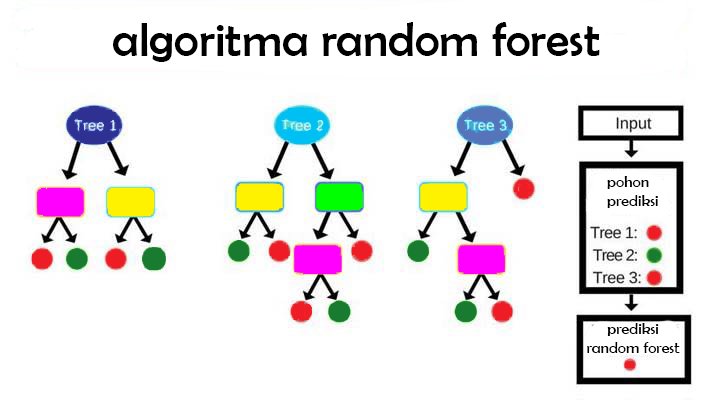
\includegraphics[width=12cm]{figures/1174075/3/1.png}
	\caption{contoh random forest}
\end{figure}


\subsubsection{Jelaskan cara membaca dataset kasus dan artikan makna setiap file dan isi field masing masing file.}
\hfill\\
Dataset adalah kumpulan data. Paling umum satu data set sesuai dengan isi tabel database tunggal, atau matriks data statistik tunggal, dimanasetiapkolomtabelmewakilivariabeltertentu,dansetiapbarissesuaidengan anggota tertentu dari dataset yang dipertanyakan.
\begin{enumerate}
\item cara membaca dataset
\hfill\\
	\begin{itemize}
	\item Gunakan librari Pandas pada python untuk dapat membaca dataset dengan format text file.
	\item Setelah itu,buat variabel baru ”dataset” yang berisikan perintah untuk membaca file csv. seperti berikut
	\hfill\\
	\lstinputlisting[firstline=8, lastline=11]{src/1174075/src3/1174070.py}
	Pada kodingan diatas dapat dijelaskan bahwa : Memanggil Librari Panda untuk membaca dataset Membuat variabel ”Dataset” yang berisikan pd.read\_csv untu kmembaca dataset.
	
	\item setelah di run maka hasilnya seperti berikut
	\hfill\\
\begin{figure}[H]
	\centering
	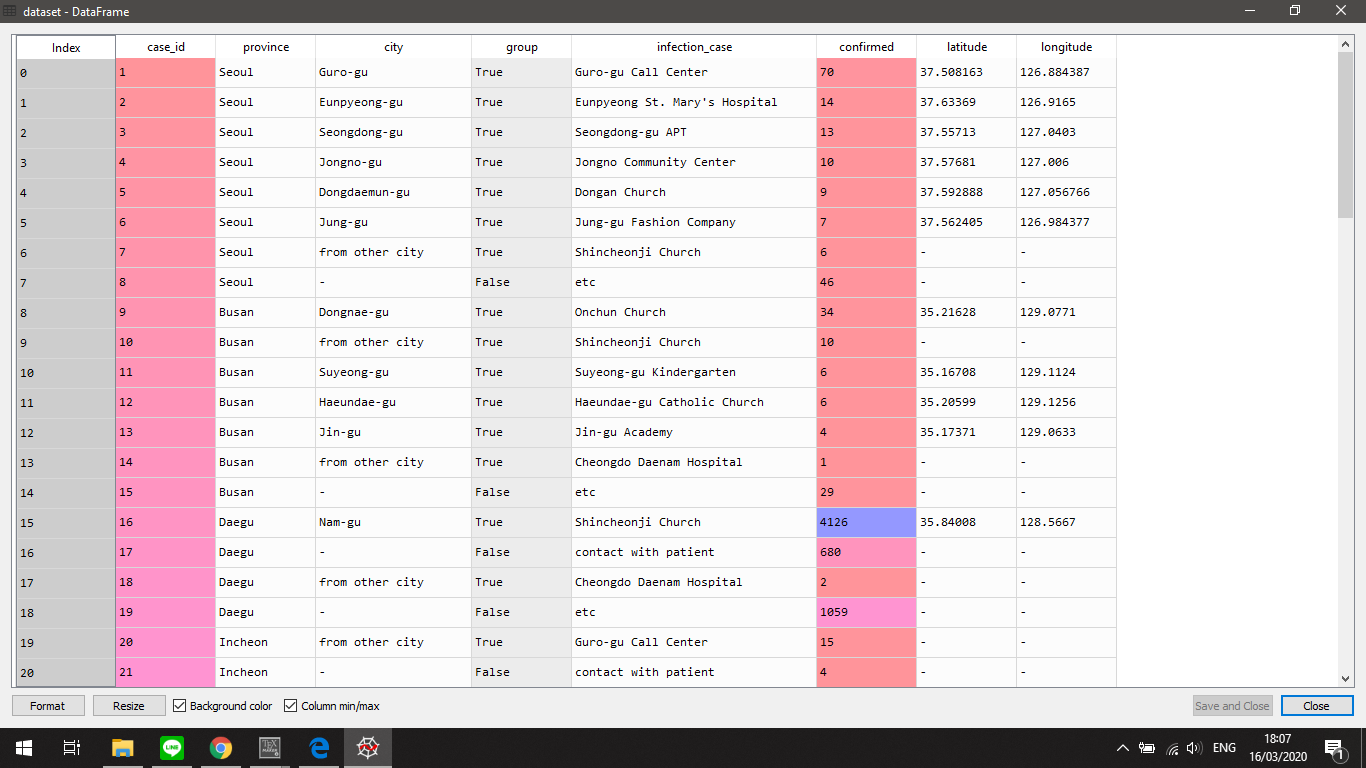
\includegraphics[width=12cm]{figures/1174075/3/2.png}
	\caption{contoh dataset}
\end{figure}
	
	Pertama tama gambar diatas merupakan dataset yang digunakan untuk mengetahui penyebaran virus corona di negara korea selatan. Datasetnya dapat didapatkan dari laman https://www.kaggle.com/kimjihoo/coronavirusdataset/data. Penjelasan dari isi field diatas adalah sebagai berikut :
	\begin{itemize}
	\item Atribut Index merupakan atribut otomatis untuk penomoran data yang ada. 
	\item Atribut case\_id merupakan nomor id dari case
	\item Atribut province merupakan nama provinsi
	\item Atribut city merupakan nama kota
	\item Atribut group terdiri dari dua variable, yaitu TRUE (untuk terindikasi infeksi dari group) dan FALSE(sebaliknya)
	\item Atribut infection\_case merupakan nama kasus yang menginfeksi
	\item Atribut confirmed merupakan kasus yang sudah terkonfirmasi
	\item Atribut latitude merupakan titik koordinat
	\item Atribut longitude merupakan titik koordinat
	\end{itemize}
	\end{itemize}
\end{enumerate}

\subsubsection{ Jelaskan apa itu cross validation}
\hfill\\
Cross-validation (CV) adalah metode statistik yang dapat digunakan untuk mengevaluasi kinerja model atau algoritma dimana data dipisahkan menjadi dua subset yaitu data proses pembelajaran dan data validasi / evaluasi. Model atau algoritma dilatih oleh subset pembelajaran dan divalidasi oleh subset validasi. Selanjutnya pemilihan jenis CV dapat didasarkan pada ukuran dataset. Biasanya CV K-fold digunakan karena dapat mengurangi waktu komputasi dengan tetap menjaga keakuratan estimasi.
	Teknik ini utamanya digunakan untuk melakukan prediksi model dan memperkirakan seberapa akurat sebuah model prediktif ketika dijalankan dalam praktiknya. Dalam sebuah masalah prediksi, sebuah model biasanya diberikan kumpulan data (dataset) yang diketahui untuk digunakan dalam menjalankan pelatihan (dataset pelatihan), serta kumpulan data yang tidak diketahui (atau data yang pertama kali dilihat)  terhadap model yang diuji (pengujian dataset) Metode 3 - fold cross validation membagi sebuah himpunan contoh  secara  acak  menjadi  3  subset yang saling bebas. Dilakukan pengulangan sebanyak 3kali untuk pelatihan dan pengujian. Pada setiap ulangan, disisakan satu subset untuk pengujian dan subset lainnya untuk pelatihan. Tingkat akurasi dihitung dengan membagi jumlah keseluruhan klasifikasi  yang benar dengan jumlah  semua  i nstance pada data  awal.

\subsubsection{Jelaskan apa arti score 44\% pada random forest, 27\% pada decission tree dan 29\% dari SVM.}
\hfill\\
Itu merupakan presentase keakurasian prediksi yang dilakukan pada saat testing menggunakan label pada dataset yang digunakan. Score merupakan mendefinisikan aturan evaluasi model. Maka pada saat dijalankan akan muncuk persentase tersebut yang menunjukan keakurasian atau keberhasilan dari prediksi yang dilakukan. Jika menggunakan Random Forest maka hasilnya 40\% , jika menggunakan Decission Tree hasil prediksinya yaitu 27\% dan pada SVM 29\% .

\subsubsection{Jelaskan bagaimana cara membaca confusion matriks dan contohnya memakai gambar atau ilustrasi sendiri.}
\hfill\\
Perthitungan Confusion Matriks dapat dilakukan sebagai berikut. Disini saya menggunakan data yang dibuat sendiri untuk menampilkan data aktual dan prediksi.
\begin{itemize}
\item Import librari Pandas, Matplotlib, dan Numpy.
\item Buat variabel y actu yang berisikan data aktual.
\item Buat variabel y pred berisikan data yang akan dijadikan sebagai prediksi.
\item Buat variabel df\_confusion yang berisikan crosstab untuk membangun tabel tabulasi silang yang dapat menunjukkan frekuensi kemunculan kelompok data tertentu.
\item Pada variabel df\_confusion definisikan lagi nama baris yaitu Actual dan kolomnya Predicted
\item Kemudian definisikan suatu fungsi yang diberi nama plot\_confusion\_matrix yang berisikan pendefinisian confusion matrix dan juga akan di plotting. untuk code lengkapnya sebagai berikut:
\lstinputlisting[firstline=14, lastline=32]{src/1174075/src3/1174075.py}
\end{itemize}
Hasil dari kode diatas akan menghasilkan confusion matrix seperti berikut:
\begin{figure}[H]
	\centering
	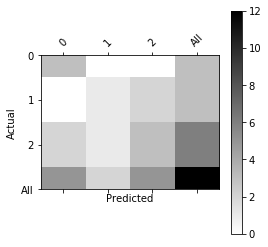
\includegraphics{figures/1174075/3/4.png}
	\caption{hasil confusion matrix}
\end{figure}

\subsubsection{Jelaskan apa itu voting pada random forest disertai dengan ilustrasi gambar sendiri.}
\hfill\\
Voting yaitu suara untuk setiap target yang diprediksi pada saat melakukan Random Forest. Pertimbangkan target prediksi dengan voting tertinggi sebagai prediksi akhir dari algoritma random forest. contohnya pada gambar berikut, dimana ada 9 hasil yang berbeda dari decision tree, dan menghasilkan suatu random forest
\begin{figure}[H]
	\centering
	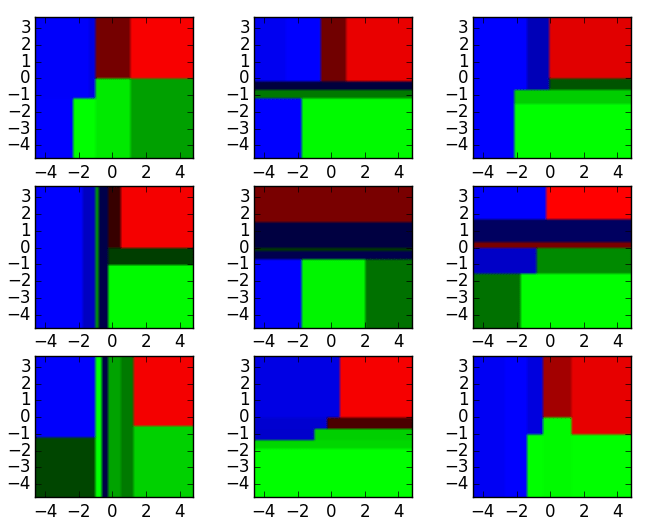
\includegraphics[width=8cm]{figures/1174075/3/5.png}
	\caption{contoh 9 hasil decision tree yang berbeda}
\end{figure}
\begin{figure}[H]
	\centering
	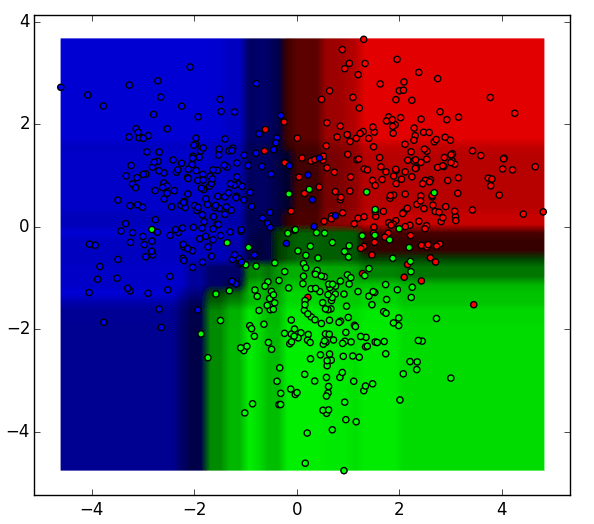
\includegraphics[width=6cm]{figures/1174075/3/6.png}
	\caption{contoh random forest}
\end{figure}

\subsection{Praktek}
\subsubsection{buat aplikasi sederhana menggunakan pandas dan jelaskan arti setiap baris kode yang dibuat(harus beda dengan teman sekelas)}
\hfill\\
Disini saya akan membuat program sederhana menggunakan Pandas yaitu untuk memilih baris dari DataFrame yang diberikan berdasarkan value disalah satu kolom. 
\lstinputlisting[firstline=8, lastline=14]{src/1174075/src3/praktek1.py}
Dari code diatas dapat dijelaskan perbarisnya sebagai berikut : 
\begin{itemize}
\item Baris pertama, yaitu import pandas yang artinya kita akan mengimport librari Pandas dari python dengan inisiasi pd.
\item Variabel d didefinisikan sebagai data. data untuk col1, col2, dan col3.
\item Variabel df akan mengubah data pada variabel d disejajarkan menjadi baris dan kolom dengan menggunakan fungsi pd.DataFrame(data=d).
\item Baris selanjutnya yaitu akan mencetak atau menampilkan tulisan "nomor 1" dan juga "Hasil: " pada jendela console
\item print(df) artinya akan mencetak atau menampilkan DataFrame dari data yang telah dibuat tadi.
\end{itemize}
Hasilnya seperti berikut:
\begin{figure}[H]
	\centering
	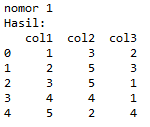
\includegraphics[width=6cm]{figures/1174075/3/7.png}
	\caption{contoh aplikasi sederhana menggunakan pandas}
\end{figure}

\subsubsection{buat aplikasi sederhana menggunakan numpy dan jelaskan arti dari setiap baris kode yang dibuat(harus beda dengan teman sekelas)}
\hfill\\
Disini saya akan membuat program sederhana menggunakan numpy, dimana saya membuat array dari angka 1 sebanyak 26 data, artinya dari angka 1-25. dan mengubah array tersebut menjadi matrix 5x5.
\lstinputlisting[firstline=16, lastline=20]{src/1174075/src3/praktek1.py}
Dari code diatas dapat dijelaskan perbarisnya sebagai berikut : 
\begin{itemize}
\item baris pertama kita meng-import numpy dan menamainya dengan np
\item lalu kita membuat variabel slur dengan diisi arraya yang dimulai dari angka 1 sebanyak 26 data(sampai angka 25) lalu mengubahnya kedalam bentuk matrix 5x5
\item Baris selanjutnya yaitu akan mencetak atau menampilkan tulisan "nomor 2" pada jendela console
\item print(slur) artinya akan mencetak atau menampilkan data yang ada pada variable slur
\end{itemize}
Hasilnya seperti berikut:
\begin{figure}[H]
	\centering
	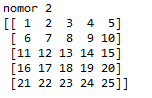
\includegraphics[width=6cm]{figures/1174075/3/8.png}
	\caption{contoh aplikasi sederhana menggunakan numpy}
\end{figure}

\subsubsection{buat aplikasi sederhana menggunakan matplotlib dan jelaskan arti dari setiap baris kode(harus beda dengan teman sekelas)}
\hfill\\\\
Disini saya akan membuat program sederhana menggunakan matplotlib.
\lstinputlisting[firstline=23, lastline=28]{src/1174075/src3/praktek1.py}
Dari code diatas dapat dijelaskan perbarisnya sebagai berikut : 
\begin{itemize}
\item baris pertama kita meng-import matplotlib.pyplot dan menamainya denan plt
\item membuat variable t dan mengisi datanya dengan array(menggunakan library numpy) yang dimulai dari angka 0 sebanyak 5 array dengan interval 0.2 untuk setiap arraynya.
\item Baris selanjutnya yaitu akan mencetak atau menampilkan tulisan "nomor 3" pada jendela console
\item plt.plot akan membuat grafik dengan data yang ada pada variable t. 'r--' itu untuk membuat garis putus-putus berwarna merah, t**2 itu sama dengan t pangkat 2, 'bo' sama dengan black oval, 'g\^' sama dengan segitiga berwarna hijau.
\item plt.show() digunakan untuk menampilkan grafik pada saat skrip dijalankan. 
\end{itemize}
Hasilnya seperti berikut:
\begin{figure}[H]
	\centering
	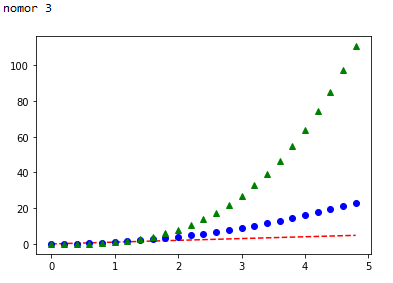
\includegraphics[width=12cm]{figures/1174075/3/9.png}
	\caption{contoh aplikasi sederhana menggunakan matplotlib}
\end{figure}

\subsubsection{jalankan program klasifikasi Random Fores pada bagian teori bab ini. Tunjukkan keluarannya dari komputer sendiri dan artikan maksud setiap luaran yang didapatkan.}
\hfill\\
Pertama dataset kita baca terlebih dahulu. 
\lstinputlisting[firstline=7, lastline=12, caption={Membaca data file txt},captionpos=b]{src/1174075/src3/bird-identifier.py}
Hasilnya seperti berikut:
\begin{figure}[H]
	\centering
	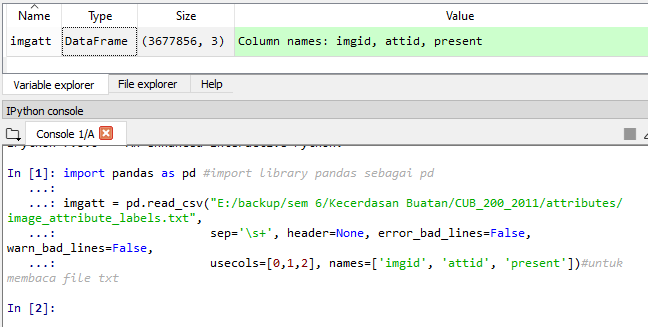
\includegraphics[width=8cm]{figures/1174075/3/10.png}
	\caption{Hasil dari listing 3.1}
\end{figure}

Melihat sebagian data awal, dengan menggunakan listing 3.2
\lstinputlisting[firstline=16, lastline=16, caption={Melihat sebagian data(bagian awal)},captionpos=b]{src/1174075/src3/bird-identifier.py} 
Hasilnya seperti berikut:
\begin{figure}[H]
	\centering
	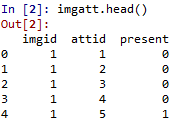
\includegraphics[width=4cm]{figures/1174075/3/11.png}
	\caption{Hasil dari listing 3.2}
\end{figure}

Melihat jumlah data menggunakan listing 3.3
\lstinputlisting[firstline=20, lastline=20, caption={Mengetahui jumlah data},captionpos=b]{src/1174075/src3/bird-identifier.py}
Hasilnya seperti berikut:
\begin{figure}[H]
	\centering
	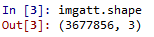
\includegraphics[width=4cm]{figures/1174075/3/12.png}
	\caption{Hasil dari listing 3.3}
\end{figure}

Merubah atribut menjadi kolom dengan menggunakan pivot layaknya excel. lalu kita cek isinya dengan menggunakan perintah pada listing 3.4
\lstinputlisting[linerange={24-24,28-28,32-32}, caption={Pivot dataset},captionpos=b]{src/1174075/src3/bird-identifier.py}
Hasilnya seperti berikut:
\begin{figure}[H]
	\centering
	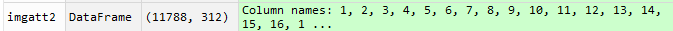
\includegraphics[width=8cm]{figures/1174075/3/13.png}
	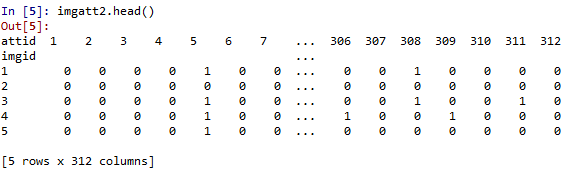
\includegraphics[width=12cm]{figures/1174075/3/13a.png}
	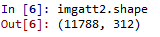
\includegraphics{figures/1174075/3/13b.png}
	\caption{Hasil dari listing 3.4}
\end{figure}

Sekarang kita akan meload jawabannya yang berisi apakah burung itu termasuk dalam spesies yang mana. Dua kolomnya adalah imgid dan label. Dan melakukan pivot yang mana imgid menjadi index yang artinya unik perintahnya ada di listing 3.5. Lalu kita cek kembali datanya. 
\lstinputlisting[linerange={36-39,43-43,47-47}, caption={Membaca dataset label file txt},captionpos=b]{src/1174075/src3/bird-identifier.py}
Hasilnya seperti berikut:
\begin{figure}[H]
	\centering
	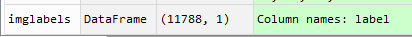
\includegraphics{figures/1174075/3/14.png}
	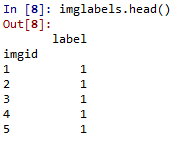
\includegraphics{figures/1174075/3/14a.png}
	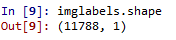
\includegraphics{figures/1174075/3/14b.png}
	\caption{Hasil dari listing 3.5}
\end{figure}

Karena isinya sama kita bisa melakukan join antara dua data. Sehingga kita akan mendapatkan data ciri dan data jawabannya atau labelnya sehingga bisa dikatekorikan supervised learning. maka perintah untuk menggabungkan kedua data dan kemudian kita melakukan pemisahan antara data set untuk training dan test dengan perintah di listing 3.6
\lstinputlisting[linerange={51-52}, caption={Menggabungkan field dari dua file terpisah},captionpos=b]{src/1174075/src3/bird-identifier.py}
Hasilnya seperti berikut:
\begin{figure}[H]
	\centering
	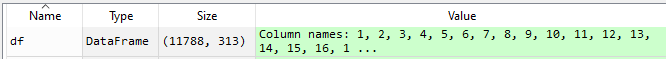
\includegraphics[width=10cm]{figures/1174075/3/15.png}
	\caption{Hasil dari listing 3.6}
\end{figure}

Kemudian drop label yang didepan, dan gunakan label yang paling belakang yang baru di join dengan perintah listing 3.7
\lstinputlisting[linerange={56-57}, caption={Memisahkan dan memilih label},captionpos=b]{src/1174075/src3/bird-identifier.py}
Hasilnya seperti berikut:
\begin{figure}[H]
	\centering
	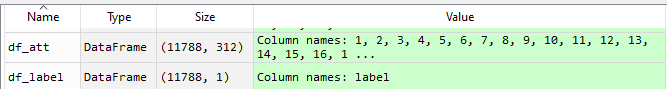
\includegraphics[width=10cm]{figures/1174075/3/16.png}
	\caption{Hasil dari listing 3.7}
\end{figure}

Kita bisa mengecek isinya dengan perintah listing 3.8
\lstinputlisting[linerange={61-61,65-65}, caption={Melihat isi masing-masing dataframe},captionpos=b]{src/1174075/src3/bird-identifier.py}
Hasilnya seperti berikut:
\begin{figure}[H]
	\centering
	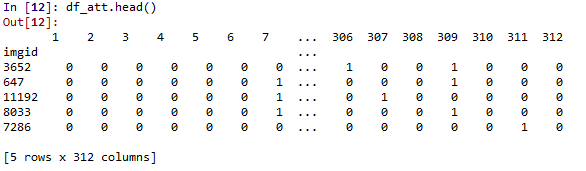
\includegraphics[width=12cm]{figures/1174075/3/17.png}
	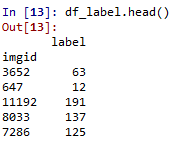
\includegraphics{figures/1174075/3/17a.png}
	\caption{Hasil dari listing 3.8}
\end{figure}

Kita bagi menjadi dua bagian, 8000 row pertama sebagai data training sisanya sebagai data testing dengan perintah listing 3.9
\lstinputlisting[linerange={69-75}, caption={Pembagian data training dan test},captionpos=b]{src/1174075/src3/bird-identifier.py}
Hasilnya seperti berikut:
\begin{figure}[H]
	\centering
	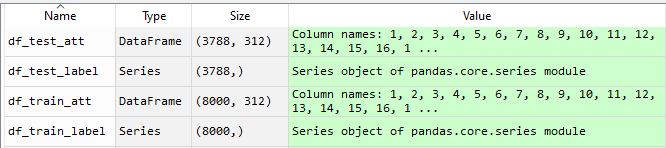
\includegraphics[width=12cm]{figures/1174075/3/18.png}
	\caption{Hasil dari listing 3.9}
\end{figure}

Kita panggil kelas RandomForestClassifier. max features diartikan sebagai berapa banyak kolom pada setiap tree dengan perintah listing 3.10
\lstinputlisting[linerange={79-80}, caption={Pembagian data training dan testInstansiasi kelas Random Forest},captionpos=b]{src/1174075/src3/bird-identifier.py}
Hasilnya seperti berikut:
\begin{figure}[H]
	\centering
	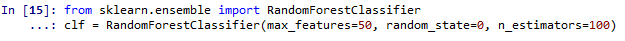
\includegraphics[width=12cm]{figures/1174075/3/19.png}
	\caption{Hasil dari listing 3.10}
\end{figure}

Kemudian lakukan fit untuk membangun random forest yang sudah ditentukan dengan maksimum fitur sebanya 50 untuk perpohonnya dengan perintah listing 3.11
\lstinputlisting[linerange={84-84}, caption={Fitting random forest dengan dataset training},captionpos=b]{src/1174075/src3/bird-identifier.py}
Hasilnya seperti berikut:
\begin{figure}[H]
	\centering
	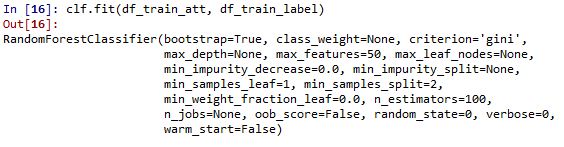
\includegraphics[width=12cm]{figures/1174075/3/20.png}
	\caption{Hasil dari listing 3.11}
\end{figure}

Hasilnya bisa kita dapatkan dengan perintah predict dengan perintah listing 3.12
\lstinputlisting[linerange={88-88}, caption={Melihat Hasil prediksi},captionpos=b]{src/1174075/src3/bird-identifier.py}
Hasilnya seperti berikut:
\begin{figure}[H]
	\centering
	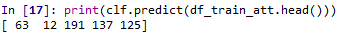
\includegraphics{figures/1174075/3/21.png}
	\caption{Hasil dari listing 3.12}
\end{figure}

Untuk besaran akurasinya dengan perintah listing 3.13
\lstinputlisting[linerange={92-92}, caption={Score perolehan dari klasifikasi},captionpos=b]{src/1174075/src3/bird-identifier.py}
Hasilnya seperti berikut:
\begin{figure}[H]
	\centering
	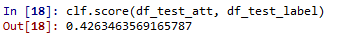
\includegraphics{figures/1174075/3/22.png}
	\caption{Hasil dari listing 3.13}
\end{figure}

\subsubsection{jalankan program confusion matrix pada bagian teori bab ini. Tunjukkan keluarannya dari komputer sendiri dan artikan maksud setiap luaran yang didapatkan.}
\hfill\\
Dari Random Forest kita coba petakan ke dalam Confusion Matrix dan lihat hasilnya dengan perintah listing 3.14
\lstinputlisting[linerange={96-98,102-102}, caption={Membuat Confusion Matrix},captionpos=b]{src/1174075/src3/bird-identifier.py}
Hasilnya seperti berikut:
\begin{figure}[H]
	\centering
	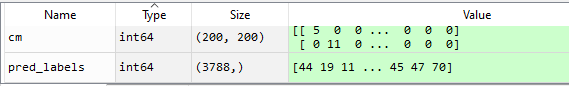
\includegraphics[width=12cm]{figures/1174075/3/23.png}
	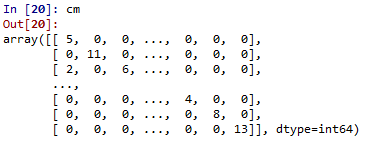
\includegraphics{figures/1174075/3/23a.png}
	\caption{Hasil dari listing 3.14}
\end{figure}

Kemudian kita plot dengan perintah
\lstinputlisting[linerange={106-136}, caption={Plotting Confusion Matrix},captionpos=b]{src/1174075/src3/bird-identifier.py}
Hasilnya seperti berikut:
\begin{figure}[H]
	\centering
	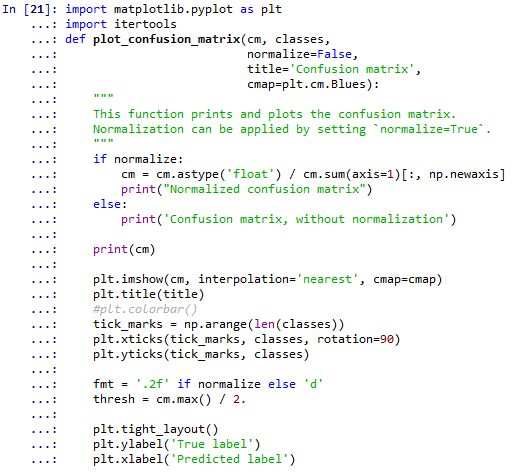
\includegraphics[width=12cm]{figures/1174075/3/24.png}
	\caption{Hasil dari listing 3.15}
\end{figure}

Agar plot sumbunya sesuai dengan nama datanya maka kita set dengan perintah
\lstinputlisting[linerange={140-143}, caption={Membaca file classes.txt},captionpos=b]{src/1174075/src3/bird-identifier.py}
Hasilnya seperti berikut:
\begin{figure}[H]
	\centering
	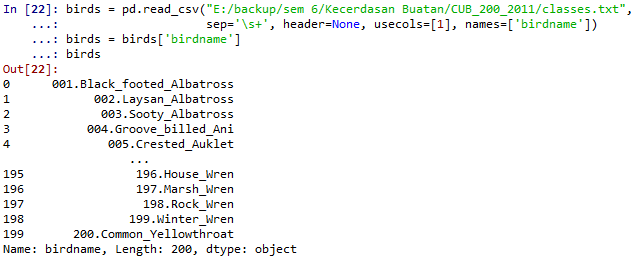
\includegraphics[width=12cm]{figures/1174075/3/25.png}
	\caption{Hasil dari listing 3.16}
\end{figure}

Lalu kita plot
\lstinputlisting[linerange={147-151}, caption={Plot hasil perubahan label},captionpos=b]{src/1174075/src3/bird-identifier.py}
Hasilnya seperti berikut:
\begin{figure}[H]
	\centering
	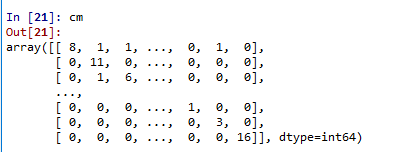
\includegraphics[width=12cm]{figures/1174075/3/26.png}
	\caption{Hasil dari listing 3.17}
\end{figure}

\subsubsection{jalankan program klasifikasi SVM dan Decission Tree pada bagian teori bab ini. Tunjukkan keluarannya dari komputer sendiri dan artikan maksud setiap luaran yang didapatkan.}
\hfill\\
Kita coba menggunakan Decission tree
\lstinputlisting[linerange={155-158}, caption={Mencoba klasifikasi dengan decission tree dengan dataset yang sama},captionpos=b]{src/1174075/src3/bird-identifier.py}
Hasilnya seperti berikut:
\begin{figure}[H]
	\centering
	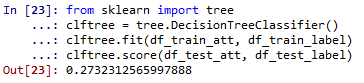
\includegraphics{figures/1174075/3/27.png}
	\caption{Hasil dari listing 3.18}
\end{figure}

Kita coba menggunakan SVM
\lstinputlisting[linerange={162-165}, caption={Mencoba klasifikasi dengan SVM dengan dataset yang sama},captionpos=b]{src/1174075/src3/bird-identifier.py}
Hasilnya seperti berikut:
\begin{figure}[H]
	\centering
	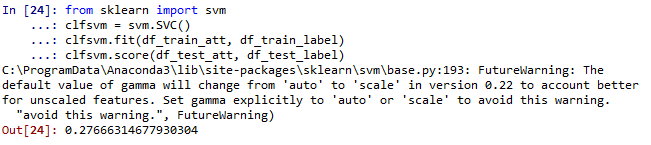
\includegraphics[width=12cm]{figures/1174075/3/28.png}
	\caption{Hasil dari listing 3.19}
\end{figure}

\subsubsection{jalankan program cross validaiton pada bagian teori bab ini. Tunjukkan keluarannya dari komputer sendiri dan artikan maksud setiap luaran yang didapatkan.}
\hfill\\
Pengeceken Cross Validation untuk Random Forest
\lstinputlisting[linerange={169-172}, caption={Hasil Cross Validation random forest},captionpos=b]{src/1174075/src3/bird-identifier.py}
Hasilnya seperti berikut:
\begin{figure}[H]
	\centering
	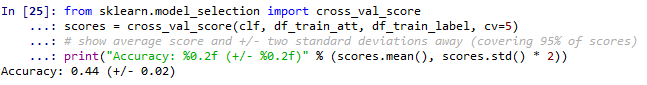
\includegraphics[width=12cm]{figures/1174075/3/29.png}
	\caption{Hasil dari listing 3.20}
\end{figure}

untuk decission tree
\lstinputlisting[linerange={176-177}, caption={Hasil Cross Validation Random Forest},captionpos=b]{src/1174075/src3/bird-identifier.py}
Hasilnya seperti berikut:
\begin{figure}[H]
	\centering
	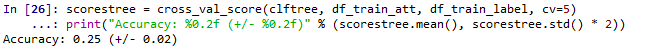
\includegraphics[width=12cm]{figures/1174075/3/30.png}
	\caption{Hasil dari listing 3.21}
\end{figure}

untuk SVM
\lstinputlisting[linerange={181-182}, caption={Hasil Cross Validation SVM},captionpos=b]{src/1174075/src3/bird-identifier.py}
Hasilnya seperti berikut:
\begin{figure}[H]
	\centering
	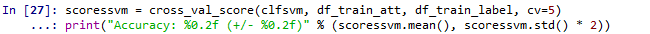
\includegraphics[width=12cm]{figures/1174075/3/31.png}
	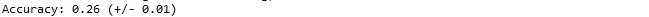
\includegraphics{figures/1174075/3/31a.png}
	\caption{Hasil dari listing 3.22}
\end{figure}

\subsubsection{jalankan program pengamatan komponen informasi pada bagian teori bab ini. Tunjukkan keluarannya dari komputer sendiri dan artikan maksud setiap luaran yang didapatkan.}
\hfill\\
Untuk mengetahui berapa banyak tree yang dibuat, berapa banyak atribut yang dipakai dan informasi lainnya menggunakan kode
\lstinputlisting[linerange={186-199}, caption={Melakukan Pengamatan komponen informasi},captionpos=b]{src/1174075/src3/bird-identifier.py}
Hasilnya seperti berikut:
\begin{figure}[H]
	\centering
	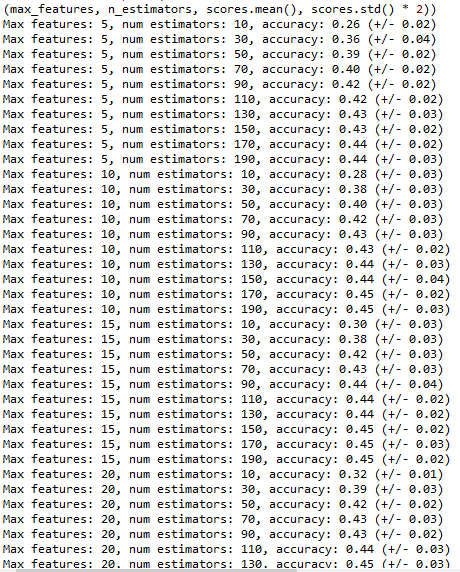
\includegraphics[width=10cm]{figures/1174075/3/32.png}
	\caption{Hasil dari listing 3.23}
\end{figure}
\begin{figure}[H]
	\centering
	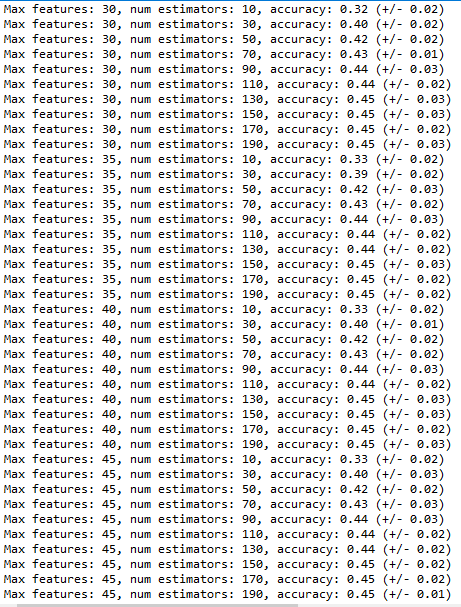
\includegraphics[width=10cm]{figures/1174075/3/32a.png}
	\caption{Hasil dari listing 3.23(2)}
\end{figure}


Dan kita bisa melakukan plot informasi ini dengan kode
\lstinputlisting[linerange={203-217}, caption={Plot Komponen informasi agar bisa dibaca},captionpos=b]{src/1174075/src3/bird-identifier.py}
Hasilnya seperti berikut:
\begin{figure}[H]
	\centering
	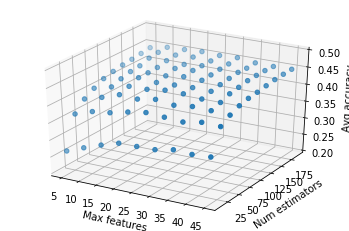
\includegraphics[width=12cm]{figures/1174075/3/33.png}
	\caption{Hasil dari listing 3.24}
\end{figure}


\subsection{Penanganan Error}
\subsubsection{skrinsut Error}
\hfill\\
Untuk Error, saya tidak menemukannya. tetapi saya mengalami not responding beberapa kali. seperti pada gambar berikut, dimana not responding terjadi karena laptop dengan spek yang minim melakukan kinerja yang sangat berat.
\begin{figure}[H]
	\centering
	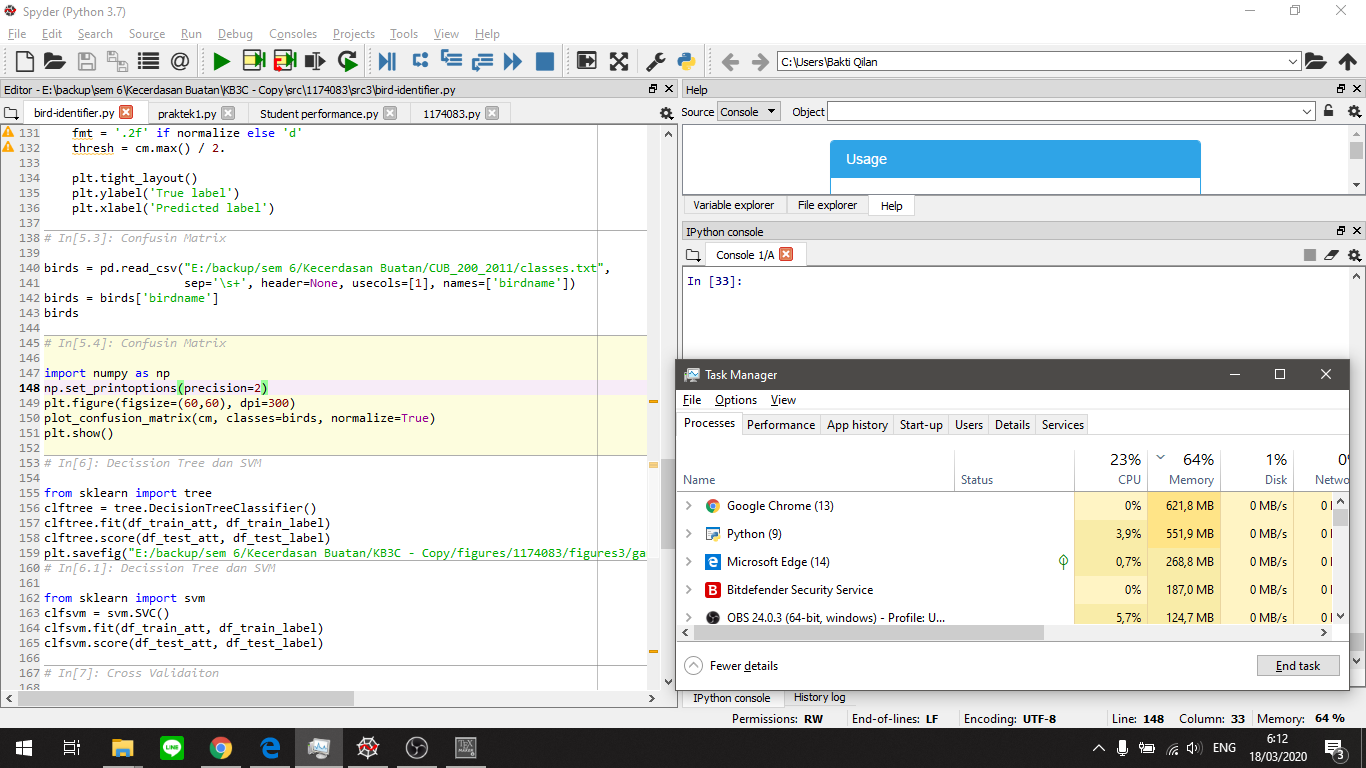
\includegraphics[width=12cm]{figures/1174075/3/error1.png}
	\caption{Before Disaster}
\end{figure}
\begin{figure}[H]
	\centering
	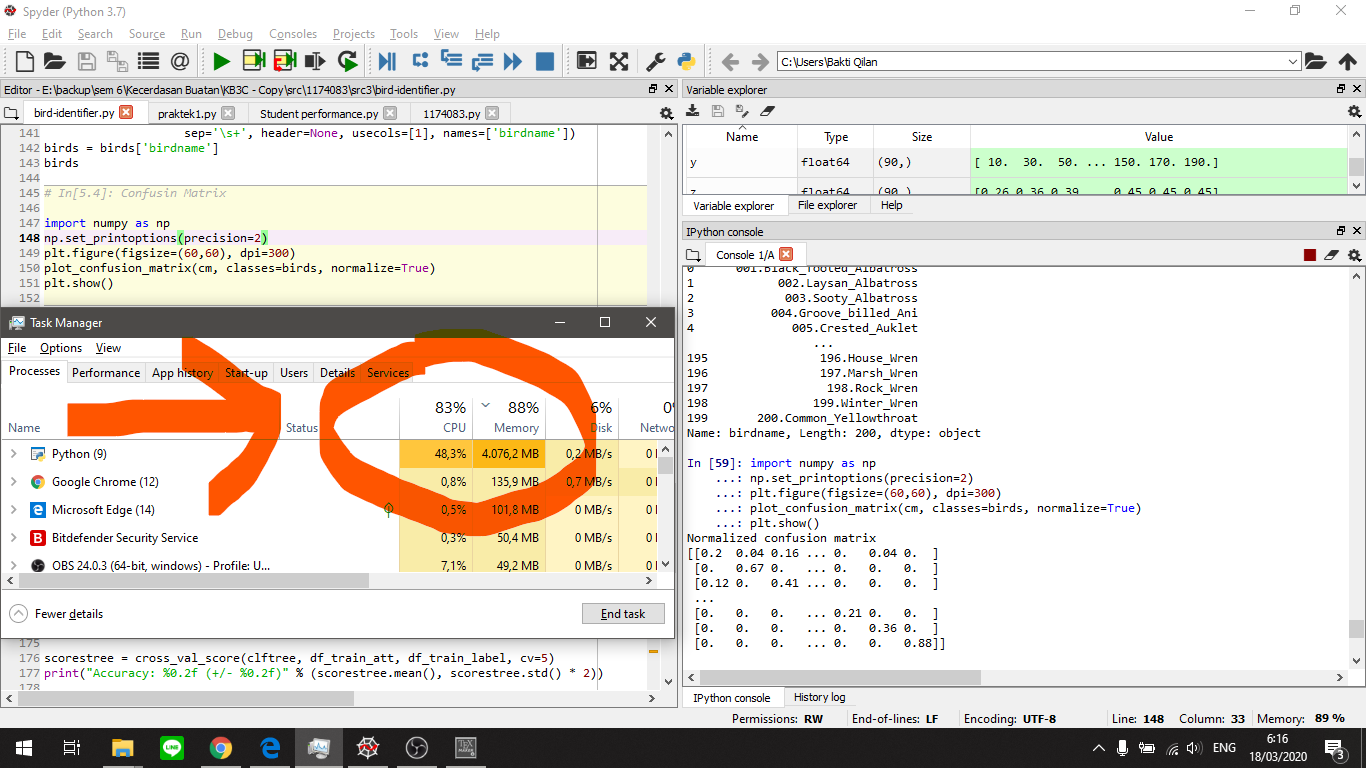
\includegraphics[width=12cm]{figures/1174075/3/error2.png}
	\caption{After Disaster}
\end{figure}

\subsubsection{Tuliskan Kode Error dan Jenis Error}
\hfill\\
\begin{figure}[H]
	\centering
	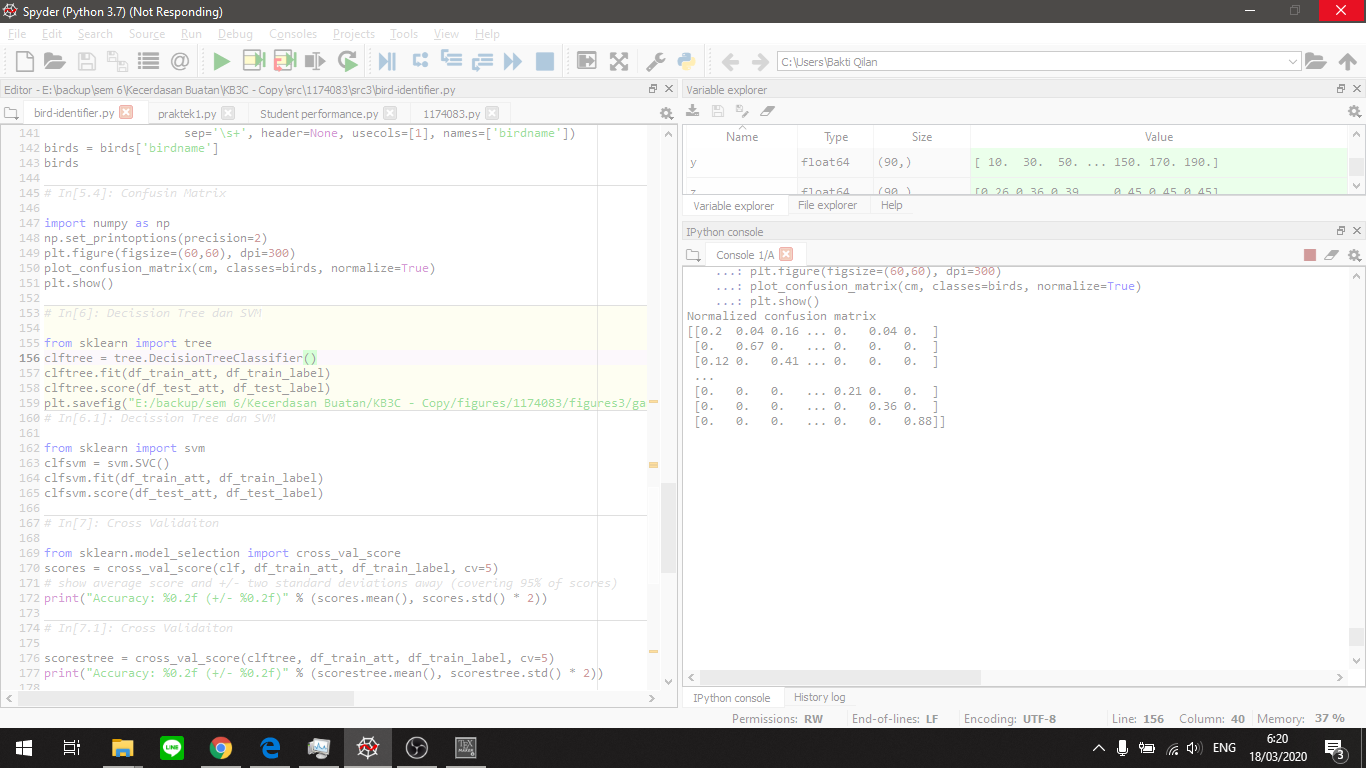
\includegraphics[width=12cm]{figures/1174075/3/error3.png}
	\caption{Not Responding pun terjadi}
\end{figure}

\subsubsection{Cara Penanganan Error}
\hfill\\
Untuk mengatasinya, saya endtask terlebih dahulu spydernya. dan memodifikasi codingannya. yang asalnya
\begin{figure}[H]
	\centering
	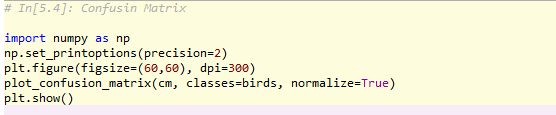
\includegraphics[width=12cm]{figures/1174075/3/error4.png}
	\caption{Sebelum diubah}
\end{figure}

\begin{figure}[H]
	\centering
	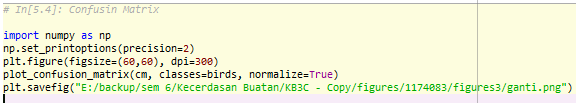
\includegraphics[width=12cm]{figures/1174075/figures3/error5.png}
	\caption{Setelah diubah}
\end{figure}
yang asalnya pada baris terakhir itu plt.show() yaitu untuk menampilkannya di console, saya ganti menjadi plt.savefig yang berfungsi menyimpan langsung gambar dari grafik tersebut. dan not respinding ini terjadi karena laptop berusaha menampilkan gambar dengan ukuran yang besar, yaitu 18000x18000px tetapi speknya hanya tidak mampu maka terjadilah not responding. tetapi jika kita hanya langsung men save figurenya maka proses akan berjalan lancar meskipun agak lama.
\begin{figure}[H]
	\centering
	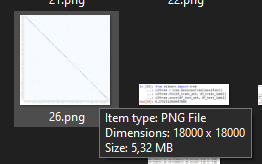
\includegraphics[width=5cm]{figures/1174075/figures3/error6.png}
	\caption{Detail Gambar Confusion Matrix}
\end{figure}
\hfill\\

\subsubsection{Bukti Tidak Plagiat}
\hfill\\
\begin{figure}[H]
	\centering
	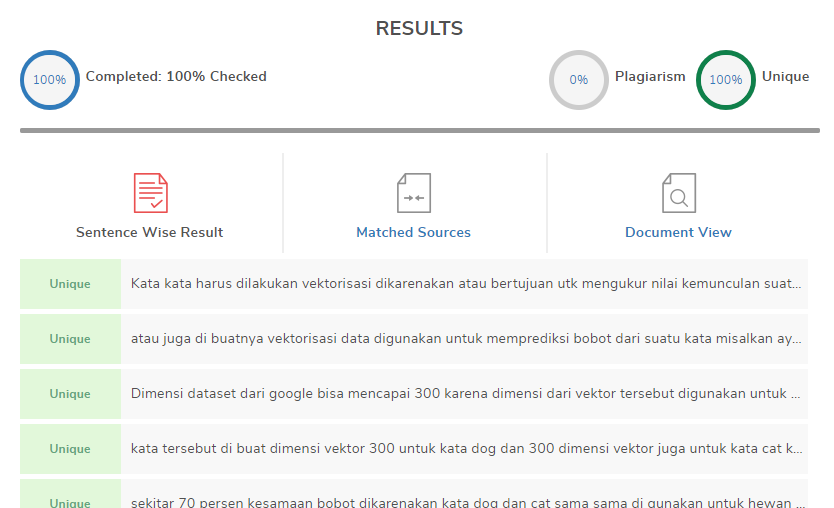
\includegraphics[width=12cm]{figures/1174075/figures3/plagiat.png}
	\caption{Cek Plagiarism}
\end{figure}
\begin{figure}[H]
	\centering
	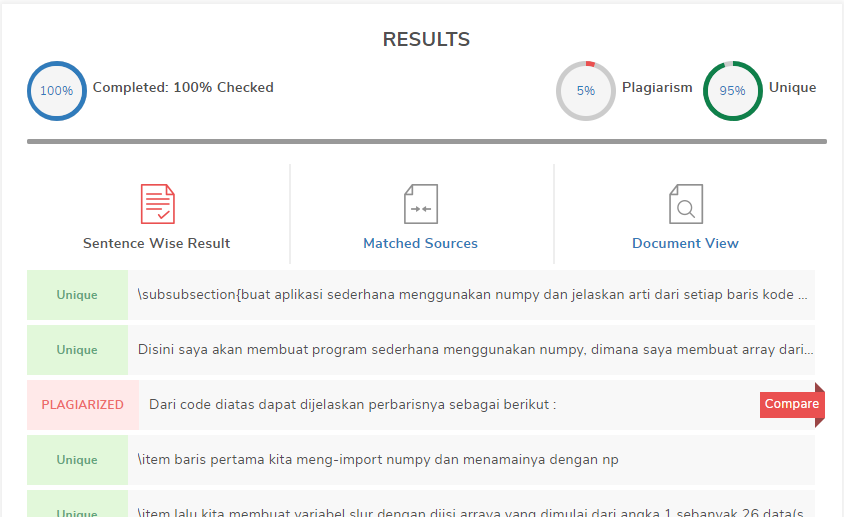
\includegraphics[width=12cm]{figures/1174075/figures3/plagiat1.png}	
	\caption{Cek Plagiarism(2)}
\end{figure}


\subsection{Link Video Youtube}
https://youtu.be/DyJRzPrFxiQ